\newpage
\section{Clock}
    Die Clock wird am einfachsten, passend aus der gewollten Baudrate für die USART ausgewählt. Damit die Baudrate richtig berechnet wird.\\
    Die HSI Clock von 8MHz ist standard mäßig aktiviert.\\
    Weiterhin werden im APB2 Bus die Clocks für die USART1 und für den ADC und im AHB Bus für die GPIO Ports aktiviert. 
    Die weiteren Clock einstellungen wie z.B. für die USART sind in der jeweilign Initiallisierungs Funktion enthalten.
    
    \begin{figure}[!htb]
        \centering
        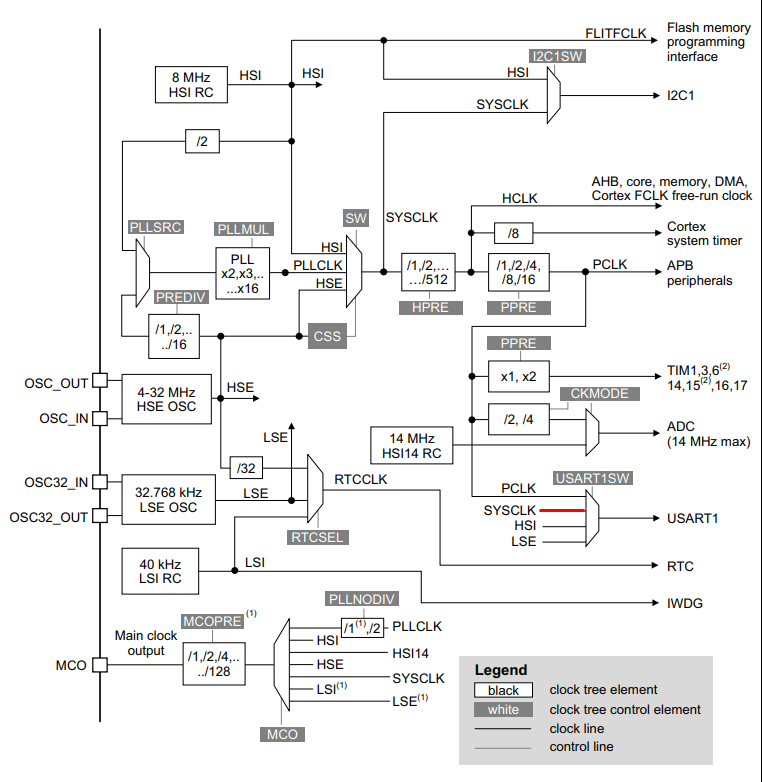
\includegraphics[scale=0.65]{Clock-Tree.png}
        \caption{Clock-Tree}
        \label{caption:Clock-Tree}
    \end{figure}
    
    
\newpage
\subsection{Clock-Code}
\begin{lstlisting}[language=C, style=CStyle, caption=init-CLOCK, captionpos=b, label=init-CLOCK]
int init_CLOCK()
{
    uint32_t reg_content;
    uint32_t* rcc_ahbenr = RCC_AHBENR; 
    uint32_t* rcc_apb2enr = RCC_APB2ENR;
    uint32_t* rcc_cfgr = RCC_CFGR;

    //GPIO A port clock enable
    reg_content = *rcc_ahbenr;
    reg_content |= 0x00020000;
    *rcc_ahbenr = reg_content;
    
    //USART1 clock enable
    reg_content = *rcc_apb2enr;
    reg_content |= 0x00004200;
    *rcc_apb2enr = reg_content;

    //set AHB Clock to not divided so same clock as sysclock
    reg_content = *rcc_cfgr;
    reg_content |= 0x00000000;
    *rcc_cfgr = reg_content; 
}
\end{lstlisting}